\documentclass{article}

\usepackage[utf8]{inputenc}
\usepackage{graphicx}

\title{Comportamento e Cuidados com Gatos Domésticos}
\author{Equipe de Estudo}
\date{\today}

\begin{document}

\maketitle

\section{Introdução}

Os gatos domésticos são animais de estimação populares em todo o mundo devido à sua independência, comportamento curioso e facilidade de adaptação. Além de serem companheiros afetivos, os gatos possuem características comportamentais únicas que despertam interesse científico e social. De acordo com \cite{gatosref}, compreender o comportamento felino é essencial para garantir seu bem-estar.

\section{Desenvolvimento}

Os gatos apresentam hábitos específicos que refletem seus instintos naturais, como a caça, o descanso prolongado e a marcação de território. Para garantir uma convivência saudável, é importante considerar alguns cuidados básicos:

\begin{itemize}
    \item Fornecer alimentação balanceada e adequada;
    \item Manter a higiene da caixa de areia;
    \item Estimular atividades físicas e brincadeiras.
\end{itemize}

A Figura 1 apresenta um exemplo ilustrativo de um gato doméstico.

\begin{figure}[h]
    \centering
    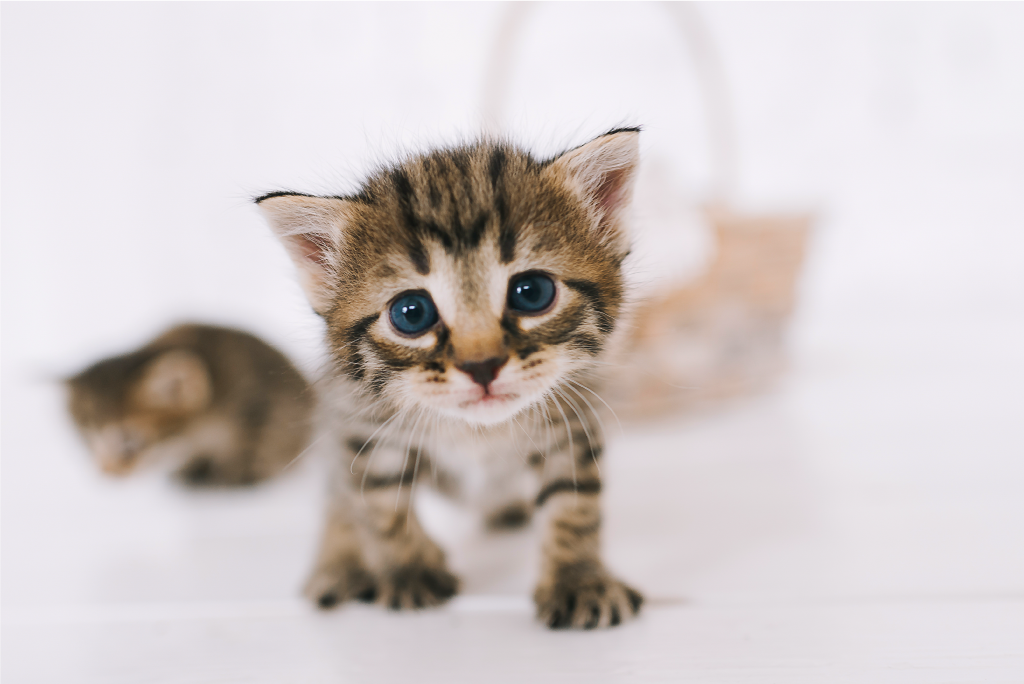
\includegraphics[width=0.5\textwidth]{gatofoto.png}
    \caption{Exemplo ilustrativo de um gato doméstico}
\end{figure}

Como mostrado na Figura 1, os gatos possuem características físicas marcantes, como agilidade e postura elegante.

Além disso, é possível organizar informações importantes sobre cuidados com gatos em forma de tabela, como na Tabela 1.

\begin{table}[h]
\centering
\begin{tabular}{|c|c|}
\hline
Cuidado & Descrição \\
\hline
Alimentação & Ração balanceada e água fresca \\
Higiene & Limpeza regular da caixa de areia \\
Saúde & Consultas veterinárias periódicas \\
\hline
\end{tabular}
\caption{Cuidados básicos com gatos domésticos}
\end{table}

A Tabela 1 resume práticas essenciais para manter a saúde e o bem-estar dos gatos.

\section{Conclusão}

Os gatos domésticos são animais que exigem atenção, mesmo sendo independentes. Compreender seu comportamento e oferecer cuidados adequados são fatores fundamentais para uma convivência harmoniosa. Dessa forma, a relação entre humanos e gatos se torna mais saudável e satisfatória.

\begin{thebibliography}{9}

\bibitem{gatosref}
Autor Fictício. \textit{Manual de Cuidados com Gatos Domésticos}. Editora Animal, 2021.

\end{thebibliography}

\end{document}
